\section{Implementation}
I have identified three systems that compromise the project:
\begin{mylist}
  \item The Hardware, Mechanics and Electronics
  \item The software that coordinates the various components
  \item The Computer Vision system
\end{mylist}

\noindent
For the first version of the system and before a comprehensive literature review was conducted, I initially designed
the system to use a face-up camera that would identify components placed on an acrylic plate directly above it. 
This design was chosen as it was the simplest design that would allow for component identification and could 
be easily implemented using the resources available to me. Additionally, the camera used in the system came with
a short ribbon cable, which limited the distance between the camera and the Pi, which would have made the face-down
design more difficult to reasonably implement.

In the following sections, I will discuss the implementation of each of these systems.

% Hardware
\include*{subpages/Hardware}
% Figures for 3D Printed Frame
\begin{figure*}
  \begin{minipage}[t]{0.32\textwidth}
    \centering
    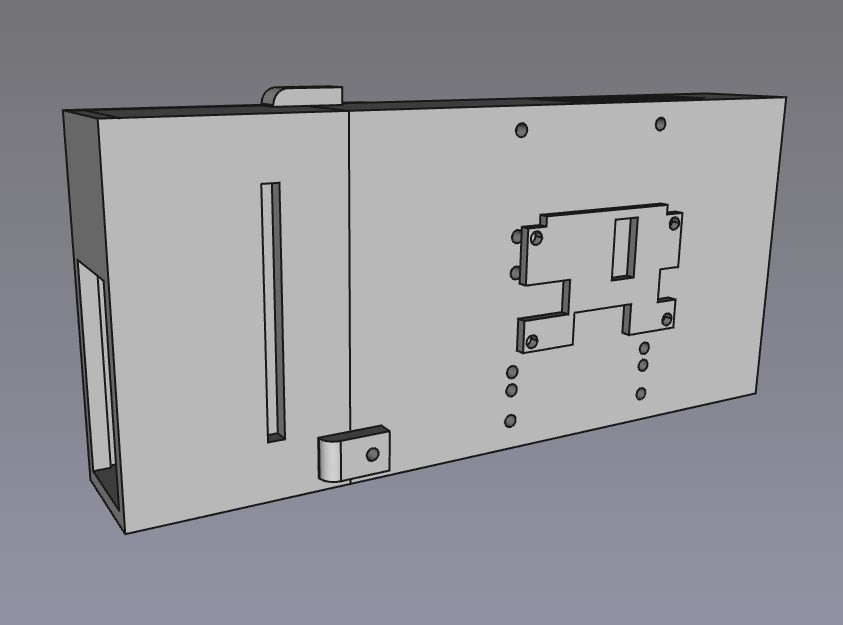
\includegraphics[width=\textwidth,height=5cm]{imgs/freecad/psu_mount.jpg}
    \caption{PSU Housing}
  \end{minipage}
  \hfill
  \begin{minipage}[t]{0.32\textwidth}
    \centering
    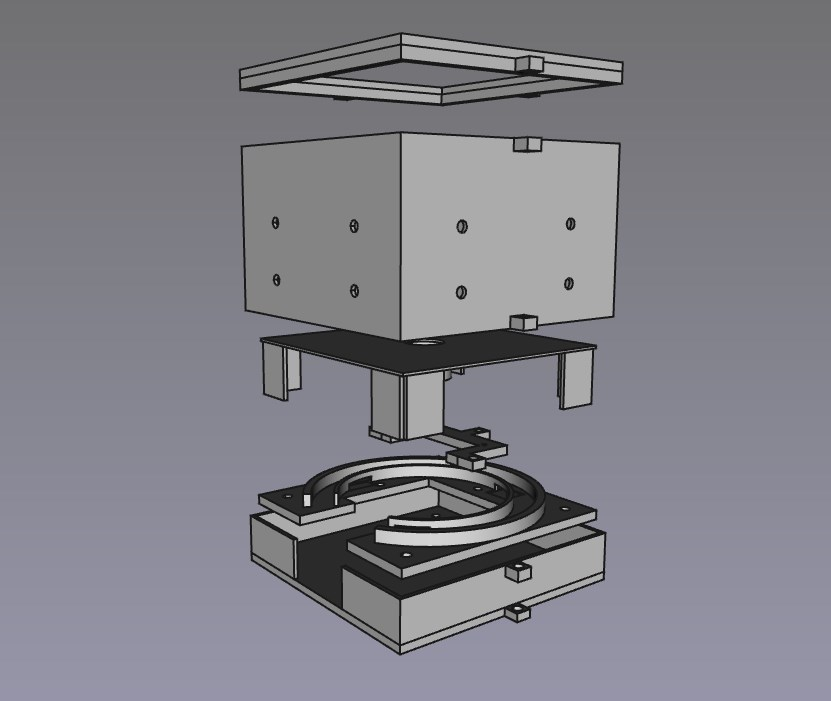
\includegraphics[width=\textwidth,height=5cm]{imgs/freecad/camera_case.jpg}
    \caption{Camera Housing}
    \label{fig:camerahousing}
  \end{minipage}
  \hfill
  \begin{minipage}[t]{0.32\textwidth}
    \centering
    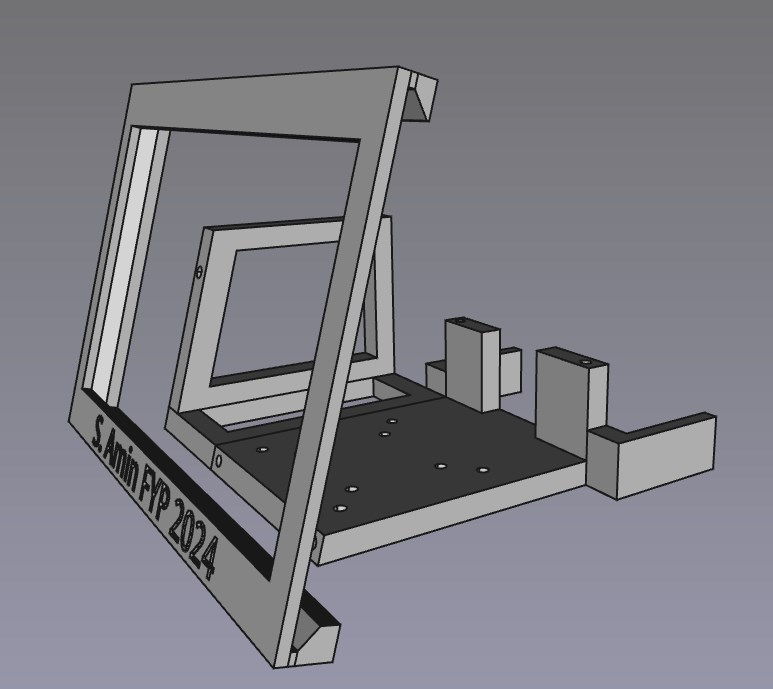
\includegraphics[width=\textwidth,height=5cm]{imgs/freecad/lcd_mount.jpg}
    \caption{LCD Display Housing}
  \end{minipage}
\end{figure*}

% 3D Printed Frame
\include*{subpages/Mechanics}

% Electronics
\include*{subpages/Electronics}

% Design Problems
\include*{subpages/Design Problems}

% Software
\include*{subpages/Software}

% Computer Vision
\include*{subpages/Computer Vision}

